\documentclass[11pt,a4paper]{scrartcl}
\usepackage[margin=2cm]{geometry}
\setlength{\parskip}{5pt}
% Encoding
\usepackage[utf8]{inputenc}
% Bibliography
\usepackage[backend=biber,bibstyle=ieee,citestyle=numeric]{biblatex}
\bibliography{coms10005_cw2}
\usepackage[hidelinks]{hyperref} % Clickable links
% Header
\usepackage{fancyhdr}
\pagestyle{fancy}
\lhead{COMS10005 Coursework 2}
\rhead{}
%Figures
\usepackage{graphicx}
\graphicspath{ {images/} }
\usepackage{subfig}
%Per page footnote numbering
\usepackage[perpage]{footmisc}

\begin{document}
	
\section*{Password Security: KeePass Password Safe}
\begin{refsection}

There are a number of recommendations that should be followed in order to use passwords securely. 
First of all a password needs to be sufficiently long and complex (i.e. drawn from a large set of characters) to make a brute force attack infeasible. Especially in the absence of rate-limiting or account blocking after failed attempts; such as when using poorly developed applications or if there is a possibility of an offline attack \cite{nist_password_2017}.
Secondly, dictionary words, common or previously compromised passwords, context related information (e.g. the website name), or easily obtained personal information (e.g. birthdays, phone numbers) should not be used to create a password. Otherwise the password would be vulnerable to dictionary attacks (a type of brute force attack where only likely possibilities are attempted).
Finally the password should be kept private, never stored in a plain text file or written down \cite{cern_computer_security_information}.

These requirements are further complicated by the importance of using unique passwords for different services. If one of these services were attacked and the password exposed, the attacker could gain access to any other services using the same password. There are many reasons why this could be possible, some examples include: An application failing to properly implement password hashing; perhaps using a weak algorithm, or by not using salt, making the passwords vulnerable to rainbow table attacks (a table of precomputed hash chains) \cite{linkedin_leak}. Alternatively misconfigured server logging may capture and store passwords as plain text before they even reach the hash algorithm  \cite{github_logs,twitter_logs}.

The more services that a person uses it becomes increasingly difficult for them to remember good unique passwords for each one.
Research by Experian plc found that 'people have on average up to 26 online accounts protected by only five different passwords' \cite{experian_2016}.
In my personal experience I found that I was using the same password for countless different websites, all using the same email address. 
A possible solution to this problem was to use a password manager \cite{ncsc_pass_managers}, this is a utility that removes the need to remember numerous passwords by storing them in an encrypted database accessible using a single master password\footnote{Password managers may also combine the password with other forms of authentication such as a key file.}.

I elected to use KeePass Password Safe \cite{keepass}, it has the advantage of being free and open source, although compared to premium services (such as LastPass) it does require the user to be entirely responsible for storing and synchronising the database file. Fortunately in my situation this was not a problem as I was already was self hosting a Seafile file server. This setup adds a further layer of security because not only is the KeePass database file encrypted itself with its own password, no external parties can gain access to the file because it is only stored on my own encrypted disks and it is synchronised between them over HTTPS.

When using KeePass on a desktop environment\footnote{If you use a clipboard manager (I am using Ditto for example), an exclusion should be added to prevent capturing KeePass entries, which would otherwise get saved as plaintext.} 
I have installed KeePassHttp, a plugin that exposes the database through a HTTP server, making entries accessible to browser plugins such as chromeIPass\footnote{The server is bound exclusively to the localhost / loopback interface, and an AES key stored in the database is used to encrypt the traffic between the two applications.}. Not only does browser integration improve usability it  potentially adds protection against phishing: The browser plugin will only extract entries from KeePass when the present URL matches the database value, therefore the chance of being fooled by a phishing site is reduced because I would notice that the password fields are not being populated \cite{ncsc_pass_managers}.

There is unfortunately one criticism that can be made against password managers in that they exacerbate the risk of a compromised device\footnote{Such as where an attacker has sufficient privileges to install a key logger or read the memory of another process.}.
In the absence of a password manager the attacker would have to wait until I signed in on that device (if ever) to each service they are targeting. 
Whereas as soon as I sign in to KeePass they would gain immediate access to all credentials, including those which may never have been entered on that device \cite{citadel_keepass}. Regardless both scenarios highlight the importance of maintaining good security practices on all of my devices; at the point they are totally compromised, having a strong password becomes irreverent \cite{nist_password_2017}.

\printbibliography
\end{refsection}

\newpage

\section*{Using LDAPS for centralised authentication}
\begin{refsection}

I currently have two Ubuntu servers, one running Seafile (a file server) \cite{seafile}, and another running Gogs (a Git service) \cite{gogs}. Instead of having to maintain multiple sets of credentials, I had configured these servers to centrally authenticate users using LDAP \cite{RFC4510} with my Active Directory (hereafter as AD) server. All three servers are connected to the same Ethernet network switch and VLAN. The network does not use any form of access control (such as 802.1X) and it is also accessible via Wi-Fi using a pre-shared key.

I realised that this setup created a potential security weakness because by default LDAP traffic is not encrypted \cite[sec 6.1]{RFC4513} \cite{microsoft_enable_ldaps}. For example, figure \ref{fig:wireshark_ldap} shows part of the LDAP data that is transmitted as plaintext over the network when I attempted to login to the Gogs server:

\begin{figure}[h]
	\centering
	\subfloat[Text]{{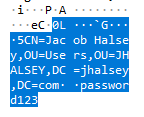
\includegraphics[width=2.5cm,keepaspectratio]{ldap_data}}}
	\qquad
	\subfloat[Details]{{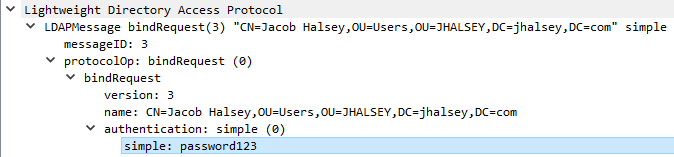
\includegraphics[width=9cm,keepaspectratio]{ldap_formatted}}}
	\caption{Wireshark capture of an LDAP bind request}
	\label{fig:wireshark_ldap}
\end{figure}

Although during normal Ethernet operation a frame sent from one node to another node will not be seen by other nodes on the network (aside from during the initial MAC learning process)\footnote{And also when using an Ethernet hub; the network functions as a bus, however these are rarely used today.}, there are at least three types of attack that could be used to manipulate the flow of Ethernet traffic between the servers\footnote{There are other types of layer 2 attacks (e.g. an STP root bridge attack), but they are not really relevant to my network configuration.}; allowing an attacker to intercept the unencrypted credentials.
These include: MAC address spoofing, CAM table overflows, and ARP spoofing\footnote{In actual fact the servers are configured to use IPv6 which does not use ARP, but rather NDP, however the concept is the same.} \cite{l2attacks}.
While there are various methods to counter these attacks, including port security tools provided on some Ethernet switches \cite[193]{odom_icnd1}.
None of these are ideal solutions for my network because the Ethernet switches do not have consistent support for these features, and it would add significant management overhead to maintain their configuration.

To solve this problem I decided to enable Secure LDAP (LDAPS), which uses TLS to authenticate and encrypt communication between the servers; should the traffic be intercepted by an attacker, they would not be able to read its content. This was possible by using the following procedure \cite{microsoft_enable_ldaps, ad_ldaps_gist}:
\begin{enumerate}
	\item Creating a root certificate (and key pair), and importing it into the trusted store of the AD server.
	\item Creating a client certificate (and key pair) signed using the root certificate, for the purpose of 'Server Authentication', with the AD server's FQDN as the subject. This certificate is then imported into the AD server's personal store for LDAPS usage.
	\item The root certificate then needs to be installed on each of the Ubuntu servers so that they can establish trust of the AD server's certificate \cite{ubuntu_ca_cert}.
	\item The Ubuntu servers can now be configured to connect securely using LDAPS on port 636 using to the AD server's FQDN.
\end{enumerate}

Whilst the communication between servers is now secured, I am no longer sure if a centralised authentication setup is the overall best approach. Now that I am using a password manager having to maintain multiple sets of credentials is of little concern to me. I am instead concerned that the attack surface has been increased because the same set of credentials are moving through software products provided by numerous different vendors, if just one of these were to be exploited, then the attacker would be able to gain a set of credentials capable of accessing all the other services \cite{huque_ldap,newington_ldap}.

\printbibliography
\end{refsection}

\end{document}